%%RNN setup

\subsection{RNN setup}
A scheme of the architecture is reported in figure~\ref{fig:RNNArchitecture} and some technical details are in table~\ref{tab:RNNArchitecture}.
\begin{table}[ht]
\centering
\begin{tabular}{c|c}
\toprule
\midrule
Epochs     & 200 but EarlyStopping Callback after 10 unchanged iterations     \\
\midrule
Dropout     & $0.3 $   \\
\midrule
LSTM Layer Activation     & $tanh $   \\
\midrule
Output Layer activation     & Sigmoid   \\
\midrule
LSTM layers     & $2$   \\
\midrule
Optimiser     & Adam   \\
\midrule
Train:Test:Validation set     & $56:30:14 \%$   \\
\midrule
\bottomrule
\end{tabular}
\caption{Technical setup of the RNN architecture. ``LSTM'' stands for long short-term memory, an RNN architecture for deep learning.}
\label{tab:RNNArchitecture}
\end{table}

\begin{figure}[ht]
       \centering
       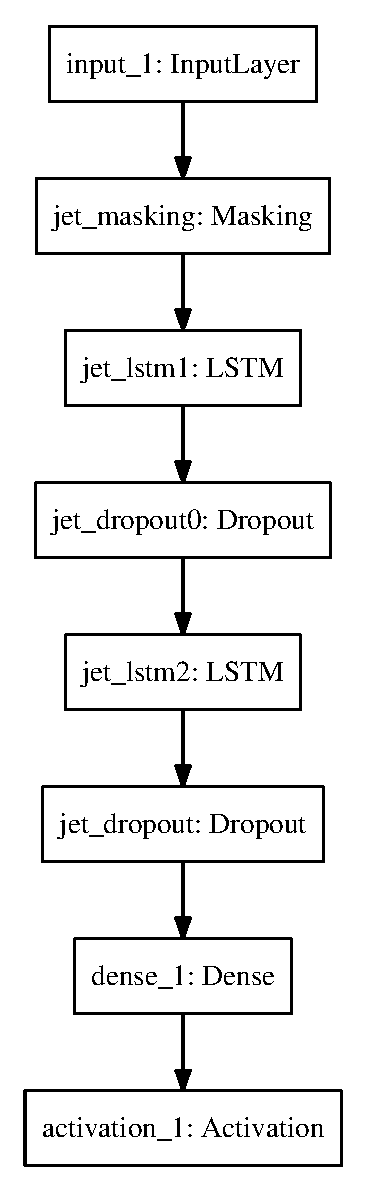
\includegraphics[width=0.15\textwidth]{figures/RNN/model.eps}
       \caption{RNN architecture scheme.}
       \label{fig:RNNArchitecture}
\end{figure}

In addition to the small-R jets information we decided to add large-R jet candidate information to further enhance the separation in the merged category; this addition is related only to the hadronically decaying boson part ($W/Z \rightarrow qq$) of the signal event topology, it is not adding anything more about the forward jets of the VBS signature.
The extra large-R informaiton is, indeed, just completing the set of information related to the VBS jets and the V-hadronic decay; in this way, the combined RNN-DNN network is able to exploit the correlation across the VBS jets and the V-hadronic of the signal topology.
The resulting architecture is schematically shown in Figure \ref{fig:RNNComboArch}.
\begin{figure}[ht]
      \centering
       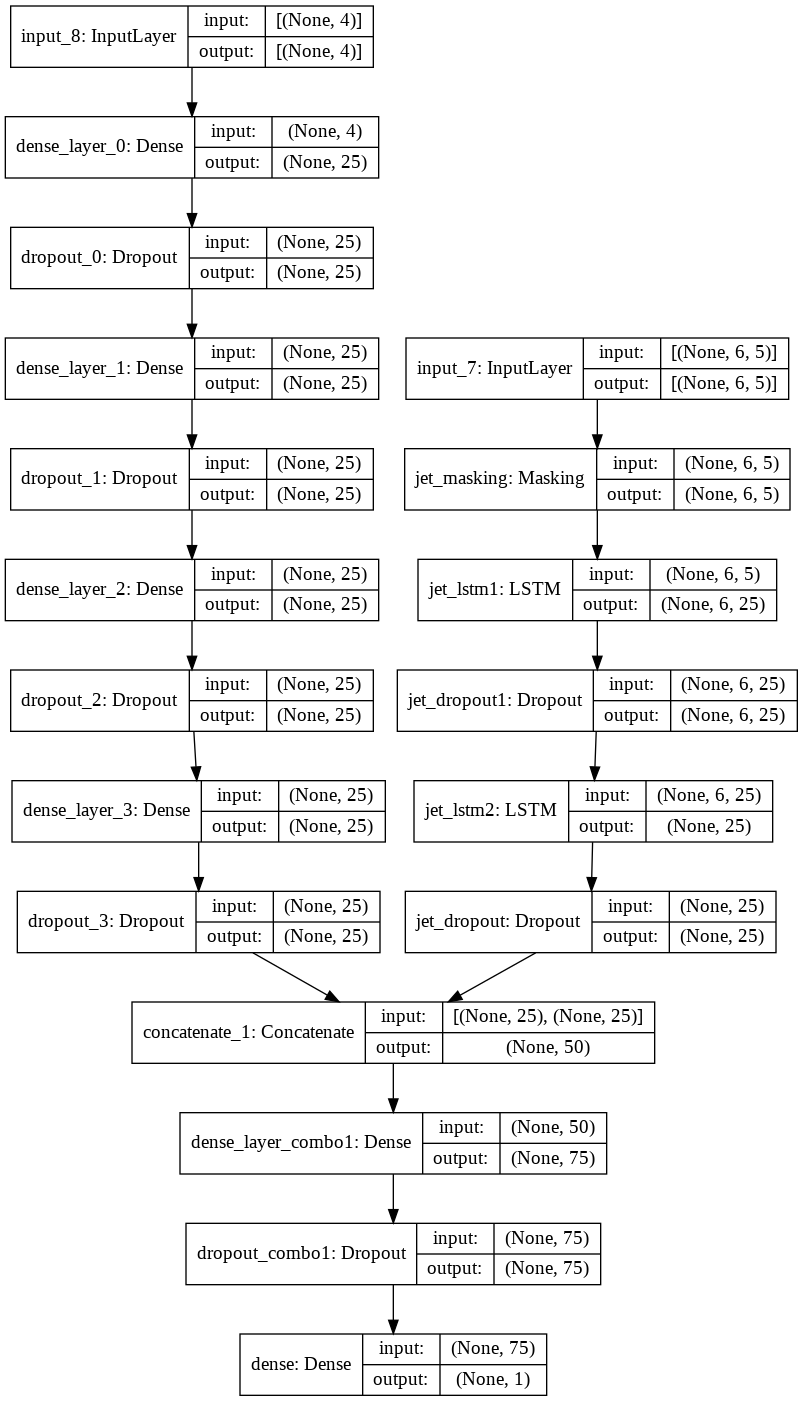
\includegraphics[width=0.5\textwidth]{figures/RNN/model_plot.png}
       \caption{Model architecture for the combined DNN + RNN based model used for the merged catigory.}
       \label{fig:RNNComboArch}
\end{figure}

